% Options for packages loaded elsewhere
% Options for packages loaded elsewhere
\PassOptionsToPackage{unicode}{hyperref}
\PassOptionsToPackage{hyphens}{url}
\PassOptionsToPackage{dvipsnames,svgnames,x11names}{xcolor}
%
\documentclass[
  ngerman,
  a4paper,
  DIV=11,
  oneside,
  openany]{scrreprt}
\usepackage{xcolor}
\usepackage{amsmath,amssymb}
\setcounter{secnumdepth}{3}
\usepackage{iftex}
\ifPDFTeX
  \usepackage[T1]{fontenc}
  \usepackage[utf8]{inputenc}
  \usepackage{textcomp} % provide euro and other symbols
\else % if luatex or xetex
  \usepackage{unicode-math} % this also loads fontspec
  \defaultfontfeatures{Scale=MatchLowercase}
  \defaultfontfeatures[\rmfamily]{Ligatures=TeX,Scale=1}
\fi
\usepackage{lmodern}
\ifPDFTeX\else
  % xetex/luatex font selection
  \setmainfont[]{Alegreya}
  \setsansfont[]{Source Sans Pro}
\fi
% Use upquote if available, for straight quotes in verbatim environments
\IfFileExists{upquote.sty}{\usepackage{upquote}}{}
\IfFileExists{microtype.sty}{% use microtype if available
  \usepackage[]{microtype}
  \UseMicrotypeSet[protrusion]{basicmath} % disable protrusion for tt fonts
}{}
\makeatletter
\@ifundefined{KOMAClassName}{% if non-KOMA class
  \IfFileExists{parskip.sty}{%
    \usepackage{parskip}
  }{% else
    \setlength{\parindent}{0pt}
    \setlength{\parskip}{6pt plus 2pt minus 1pt}}
}{% if KOMA class
  \KOMAoptions{parskip=half}}
\makeatother
% Make \paragraph and \subparagraph free-standing
\makeatletter
\ifx\paragraph\undefined\else
  \let\oldparagraph\paragraph
  \renewcommand{\paragraph}{
    \@ifstar
      \xxxParagraphStar
      \xxxParagraphNoStar
  }
  \newcommand{\xxxParagraphStar}[1]{\oldparagraph*{#1}\mbox{}}
  \newcommand{\xxxParagraphNoStar}[1]{\oldparagraph{#1}\mbox{}}
\fi
\ifx\subparagraph\undefined\else
  \let\oldsubparagraph\subparagraph
  \renewcommand{\subparagraph}{
    \@ifstar
      \xxxSubParagraphStar
      \xxxSubParagraphNoStar
  }
  \newcommand{\xxxSubParagraphStar}[1]{\oldsubparagraph*{#1}\mbox{}}
  \newcommand{\xxxSubParagraphNoStar}[1]{\oldsubparagraph{#1}\mbox{}}
\fi
\makeatother


\usepackage{longtable,booktabs,array}
\newcounter{none} % for unnumbered tables
\usepackage{calc} % for calculating minipage widths
% Correct order of tables after \paragraph or \subparagraph
\usepackage{etoolbox}
\makeatletter
\patchcmd\longtable{\par}{\if@noskipsec\mbox{}\fi\par}{}{}
\makeatother
% Allow footnotes in longtable head/foot
\IfFileExists{footnotehyper.sty}{\usepackage{footnotehyper}}{\usepackage{footnote}}
\makesavenoteenv{longtable}
\usepackage{graphicx}
\makeatletter
\newsavebox\pandoc@box
\newcommand*\pandocbounded[1]{% scales image to fit in text height/width
  \sbox\pandoc@box{#1}%
  \Gscale@div\@tempa{\textheight}{\dimexpr\ht\pandoc@box+\dp\pandoc@box\relax}%
  \Gscale@div\@tempb{\linewidth}{\wd\pandoc@box}%
  \ifdim\@tempb\p@<\@tempa\p@\let\@tempa\@tempb\fi% select the smaller of both
  \ifdim\@tempa\p@<\p@\scalebox{\@tempa}{\usebox\pandoc@box}%
  \else\usebox{\pandoc@box}%
  \fi%
}
% Set default figure placement to htbp
\def\fps@figure{htbp}
\makeatother


% definitions for citeproc citations
\NewDocumentCommand\citeproctext{}{}
\NewDocumentCommand\citeproc{mm}{%
  \begingroup\def\citeproctext{#2}\cite{#1}\endgroup}
\makeatletter
 % allow citations to break across lines
 \let\@cite@ofmt\@firstofone
 % avoid brackets around text for \cite:
 \def\@biblabel#1{}
 \def\@cite#1#2{{#1\if@tempswa , #2\fi}}
\makeatother
\newlength{\cslhangindent}
\setlength{\cslhangindent}{1.5em}
\newlength{\csllabelwidth}
\setlength{\csllabelwidth}{3em}
\newenvironment{CSLReferences}[2] % #1 hanging-indent, #2 entry-spacing
 {\begin{list}{}{%
  \setlength{\itemindent}{0pt}
  \setlength{\leftmargin}{0pt}
  \setlength{\parsep}{0pt}
  % turn on hanging indent if param 1 is 1
  \ifodd #1
   \setlength{\leftmargin}{\cslhangindent}
   \setlength{\itemindent}{-1\cslhangindent}
  \fi
  % set entry spacing
  \setlength{\itemsep}{#2\baselineskip}}}
 {\end{list}}
\usepackage{calc}
\newcommand{\CSLBlock}[1]{\hfill\break\parbox[t]{\linewidth}{\strut\ignorespaces#1\strut}}
\newcommand{\CSLLeftMargin}[1]{\parbox[t]{\csllabelwidth}{\strut#1\strut}}
\newcommand{\CSLRightInline}[1]{\parbox[t]{\linewidth - \csllabelwidth}{\strut#1\strut}}
\newcommand{\CSLIndent}[1]{\hspace{\cslhangindent}#1}

\ifLuaTeX
\usepackage[bidi=basic,shorthands=off]{babel}
\else
\usepackage[bidi=default,shorthands=off]{babel}
\fi
\ifPDFTeX
\else
\babelfont{rm}[]{Alegreya}
\fi
\ifLuaTeX
  \usepackage{selnolig} % disable illegal ligatures
\fi


\setlength{\emergencystretch}{3em} % prevent overfull lines

\providecommand{\tightlist}{%
  \setlength{\itemsep}{0pt}\setlength{\parskip}{0pt}}



 


\usepackage{booktabs}
\usepackage{longtable}
\usepackage{array}
\usepackage{multirow}
\usepackage{wrapfig}
\usepackage{float}
\usepackage{colortbl}
\usepackage{pdflscape}
\usepackage{tabularx}
\usepackage{xltabular}
\usepackage{threeparttable}
\usepackage{threeparttablex}
\usepackage[normalem]{ulem}
\usepackage{makecell}
\usepackage{xcolor}
\usepackage{booktabs}
\usepackage{longtable}
\usepackage{microtype}
\clubpenalty=10000
\widowpenalty=10000
\usepackage[font=footnotesize,labelfont={footnotesize}]{caption}
\usepackage[skins,breakable]{tcolorbox}
\definecolor{selbstviolet}{HTML}{6F42C1}
\definecolor{selbstvioletbg}{HTML}{F3EEFA}
\newtcolorbox{selbststudienphase}[1][]{
  colback=selbstvioletbg,
  colframe=selbstviolet,
  coltitle=white,
  colbacktitle=selbstviolet,
  fonttitle=\bfseries,
  breakable,
  boxrule=0.6pt,
  arc=1mm,
  title=Selbststudienphase
}
\KOMAoption{captions}{tableheading}
\makeatletter
\@ifpackageloaded{tcolorbox}{}{\usepackage[skins,breakable]{tcolorbox}}
\@ifpackageloaded{fontawesome5}{}{\usepackage{fontawesome5}}
\definecolor{quarto-callout-color}{HTML}{909090}
\definecolor{quarto-callout-note-color}{HTML}{0758E5}
\definecolor{quarto-callout-important-color}{HTML}{CC1914}
\definecolor{quarto-callout-warning-color}{HTML}{EB9113}
\definecolor{quarto-callout-tip-color}{HTML}{00A047}
\definecolor{quarto-callout-caution-color}{HTML}{FC5300}
\definecolor{quarto-callout-color-frame}{HTML}{acacac}
\definecolor{quarto-callout-note-color-frame}{HTML}{4582ec}
\definecolor{quarto-callout-important-color-frame}{HTML}{d9534f}
\definecolor{quarto-callout-warning-color-frame}{HTML}{f0ad4e}
\definecolor{quarto-callout-tip-color-frame}{HTML}{02b875}
\definecolor{quarto-callout-caution-color-frame}{HTML}{fd7e14}
\makeatother
\makeatletter
\@ifpackageloaded{bookmark}{}{\usepackage{bookmark}}
\makeatother
\makeatletter
\@ifpackageloaded{caption}{}{\usepackage{caption}}
\AtBeginDocument{%
\ifdefined\contentsname
  \renewcommand*\contentsname{Inhaltsverzeichnis}
\else
  \newcommand\contentsname{Inhaltsverzeichnis}
\fi
\ifdefined\listfigurename
  \renewcommand*\listfigurename{Abbildungsverzeichnis}
\else
  \newcommand\listfigurename{Abbildungsverzeichnis}
\fi
\ifdefined\listtablename
  \renewcommand*\listtablename{Tabellenverzeichnis}
\else
  \newcommand\listtablename{Tabellenverzeichnis}
\fi
\ifdefined\figurename
  \renewcommand*\figurename{Abbildung}
\else
  \newcommand\figurename{Abbildung}
\fi
\ifdefined\tablename
  \renewcommand*\tablename{Tabelle}
\else
  \newcommand\tablename{Tabelle}
\fi
}
\@ifpackageloaded{float}{}{\usepackage{float}}
\floatstyle{ruled}
\@ifundefined{c@chapter}{\newfloat{codelisting}{h}{lop}}{\newfloat{codelisting}{h}{lop}[chapter]}
\floatname{codelisting}{Listing}
\newcommand*\listoflistings{\listof{codelisting}{Listingverzeichnis}}
\makeatother
\makeatletter
\makeatother
\makeatletter
\@ifpackageloaded{caption}{}{\usepackage{caption}}
\@ifpackageloaded{subcaption}{}{\usepackage{subcaption}}
\makeatother
\usepackage{bookmark}
\IfFileExists{xurl.sty}{\usepackage{xurl}}{} % add URL line breaks if available
\urlstyle{same}
\hypersetup{
  pdftitle={Einführung Nachhaltige Ökonomie},
  pdflang={de},
  colorlinks=true,
  linkcolor={blue},
  filecolor={Maroon},
  citecolor={Blue},
  urlcolor={blue},
  pdfcreator={LaTeX via pandoc}}


\title{Einführung Nachhaltige Ökonomie}
\usepackage{etoolbox}
\makeatletter
\providecommand{\subtitle}[1]{% add subtitle to \maketitle
  \apptocmd{\@title}{\par {\large #1 \par}}{}{}
}
\makeatother
\subtitle{Wohlstand für alle -- innerhalb ökologischer Grenzen}
\author{}
\date{}
\begin{document}
\maketitle

\renewcommand*\contentsname{Inhaltsverzeichnis}
{
\setcounter{tocdepth}{2}
\tableofcontents
}

\bookmarksetup{startatroot}

\chapter*{Vorwort}\label{vorwort}
\addcontentsline{toc}{chapter}{Vorwort}

\markboth{Vorwort}{Vorwort}

Das folgende Skript enthält die Lernsequenzen für den Kurs
„\href{https://ilias.unibe.ch/go/crs/3443640}{Nachhaltige Ökonomie}``,
die in den Selbststudienphasen erarbeitet werden. Das Skript dient zur
Erleichterung der Bearbeitung der Sequenzen, da Ilias keine
befriedigende Lösung bietet, die Lernsequenzen herunterzuladen. Bitte
denken Sie daran, dass Sie sich an den Selbststudienphasen auf Ilias
orientieren. Dort finden Sie zusätzliche Texte, Informationen und
Übungen, die Sie bearbeiten müssen. Zudem sind viele Abschnitte
interaktiv, enthalten Links und Videos. Insgesamt enthält das Skript
sechs Kapitel, die Sie in den Selbststudienphasen 1 bis 5 erarbeiten.
Neben den Ausführungen im Skript finden Sie immer auch Hinweise auf
weiterführendes Material und Literatur. Bei Interesse können Sie dies
gerne nutzen um gewisse Themenbereiche zu vertiefen. Zur Vertiefung von
Grundfragen der Ökonomie verweisen wir gerne auf das kürzlich
erschienene Einführungslehrbuch \emph{Grundfragen der Ökonomie: Plural
-- Reflexiv -- Lebensnah} von Bäuerle et al.~(2026) (Bäuerle u.~a.
2026). Darin können Sie sich mit vielen Aspekten, die im Skript
aufgegriffen werden, vertieft auseinandersetzen. Bei Bedarf können Sie
auch jederzeit auf uns zukommen, falls Sie sich mit gewissen Themen
vertieft auseinandersetzen möchten. Wir stellen gerne weiterführendes
Material zur Verfügung.

\section*{Beitragsmatrix
(CRediT-Taxonomie)}\label{beitragsmatrix-credit-taxonomie}
\addcontentsline{toc}{section}{Beitragsmatrix (CRediT-Taxonomie)}

\markright{Beitragsmatrix (CRediT-Taxonomie)}

\begin{table}[!h]
\centering\begingroup\fontsize{8}{10}\selectfont

\begin{tabular}[t]{>{\raggedright\arraybackslash}p{2.5cm}ll>{\raggedright\arraybackslash}p{6cm}}
\toprule
\textbf{Name} & \textbf{Affiliation} & \textbf{ORCID} & \textbf{Rollen (CRediT)}\\
\midrule
\textbf{Christoph Bader} & CDE, Universität Bern & \href{https://orcid.org/0000-0002-8991-353X}{0000-0002-8991-353X} & Conceptualization, Software, Supervision, Writing – original draft, Writing – review \& editing, Project administration\\
\textbf{Nicolà Bezzola} & CDE, Universität Bern & — & Conceptualization, Writing – original draft, Writing – review \& editing\\
\textbf{Samuel Brülisauer} & CDE, Universität Bern & \href{https://orcid.org/0000-0002-2196-1922}{0000-0002-2196-1922} & Conceptualization, Writing – original draft, Writing – review \& editing\\
\bottomrule
\end{tabular}
\endgroup{}
\end{table}

\section*{Wie Sie mit diesem Skript arbeiten
können}\label{wie-sie-mit-diesem-skript-arbeiten-kuxf6nnen}
\addcontentsline{toc}{section}{Wie Sie mit diesem Skript arbeiten
können}

\markright{Wie Sie mit diesem Skript arbeiten können}

Die meisten Kapitel in diesem Skript beinhalten verschiedene
strukturierende Elemente:

\begin{tcolorbox}[enhanced jigsaw, arc=.35mm, bottomrule=.15mm, bottomtitle=1mm, breakable, colback=white, colbacktitle=quarto-callout-note-color!10!white, colframe=quarto-callout-note-color-frame, coltitle=black, left=2mm, leftrule=.75mm, opacityback=0, opacitybacktitle=0.6, rightrule=.15mm, title={Leitfragen}, titlerule=0mm, toprule=.15mm, toptitle=1mm]

Leitende Frage, an der sich das jeweilige Kapitel oder der jeweilige
Abschnitt orientiert.

\end{tcolorbox}

\begin{tcolorbox}[enhanced jigsaw, arc=.35mm, bottomrule=.15mm, bottomtitle=1mm, breakable, colback=white, colbacktitle=quarto-callout-note-color!10!white, colframe=quarto-callout-note-color-frame, coltitle=black, left=2mm, leftrule=.75mm, opacityback=0, opacitybacktitle=0.6, rightrule=.15mm, title={Vertiefungsfragen}, titlerule=0mm, toprule=.15mm, toptitle=1mm]

Für jedes Unterkapitel sind einige Vertiefungsfragen aufgeführt. Diese
dienen einerseits der selbstständigen Überprüfung des Wissens des
jeweiligen Bereichs, sollen andererseits aber auch Gedanken und
Reflexion anstossen.

\end{tcolorbox}

\begin{tcolorbox}[enhanced jigsaw, arc=.35mm, bottomrule=.15mm, bottomtitle=1mm, breakable, colback=white, colbacktitle=quarto-callout-tip-color!10!white, colframe=quarto-callout-tip-color-frame, coltitle=black, left=2mm, leftrule=.75mm, opacityback=0, opacitybacktitle=0.6, rightrule=.15mm, title={Exkurse}, titlerule=0mm, toprule=.15mm, toptitle=1mm]

Wen es genauer interessiert, darf sich in verschiedenen als solche
gekennzeichnete Exkursboxen vertiefter mit einem Thema
auseinandersetzen. Diese sind jedoch keine Pflichtlektüre.

\end{tcolorbox}

\begin{tcolorbox}[enhanced jigsaw, arc=.35mm, bottomrule=.15mm, bottomtitle=1mm, breakable, colback=white, colbacktitle=quarto-callout-caution-color!10!white, colframe=quarto-callout-caution-color-frame, coltitle=black, left=2mm, leftrule=.75mm, opacityback=0, opacitybacktitle=0.6, rightrule=.15mm, title={Weiterführende Literatur}, titlerule=0mm, toprule=.15mm, toptitle=1mm]

Vertiefende Literatur, für wer es genauer wissen will

\end{tcolorbox}

\begin{selbststudienphase}
Hier finden Sie Informationen zu den Selbststudienphasen
\end{selbststudienphase}

Das Lehrbuch \emph{Grundfragen der Ökonomie} von Bäuerle, Keil, Reinke
und Wasenitz (Hrsg.) geht auf viele besprochene Thematiken ergänzend
ein. Im Skript sind die passenden Kapitel des Lehrbuchs jeweils
erwähnt.\emph{↗ Lehrbuchkapitel 1 und 2}

\part{Nachhaltige Ökonomie}

\chapter{Wie können wir über Ökonomie
nachdenken?}\label{wie-kuxf6nnen-wir-uxfcber-uxf6konomie-nachdenken}

\begin{tcolorbox}[enhanced jigsaw, arc=.35mm, bottomrule=.15mm, bottomtitle=1mm, breakable, colback=white, colbacktitle=quarto-callout-note-color!10!white, colframe=quarto-callout-note-color-frame, coltitle=black, left=2mm, leftrule=.75mm, opacityback=0, opacitybacktitle=0.6, rightrule=.15mm, title={Leitfrage}, titlerule=0mm, toprule=.15mm, toptitle=1mm]

Was ist eigentlich Ökonomie -- und weshalb gibt es so unterschiedliche
Vorstellungen davon, was als „ökonomisch`` gilt und wie wirtschaftliches
Handeln gedacht werden sollte?

\end{tcolorbox}

\section{Was ist Ökonomie?}\label{was-ist-uxf6konomie}

\emph{↗ Lehrbuchkapitel 1 und 2}

Der Begriff der Ökonomie ist in unserem Alltag allgegenwärtig.
Ökonomische Themen nehmen beispielsweise in Zeitungen, unseren
alltäglichen Diskussionen, in politischen Debatten sowie in den sozialen
Medien einen prominenten Platz ein. Und in der Tagesschau werden Themen
verschiedentlich von Ökonom*innen aus einer \emph{ökonomischen
Perspektive} eingeordnet. Aber was ist genau diese ökonomische
Perspektive? Es erscheint schnell der Eindruck, dass alle genau wissen,
was mit dieser ökonomischen Perspektive gemeint ist. Intuitiv verbinden
wir diese häufig mit Begriffen wie Märkten, Preisen und
Finanzwirtschaft. Tatsächlich ist jedoch weder in der Geschichte des
Begriffs noch in der Gegenwart abschliessend geklärt, was mit Ökonomie
und somit dem Gegenstandsbereich der Volkswirtschaftslehre gemeint ist.
Da Volkswirtschaftslehre eine Sozialwissenschaft ist, haben wir es nicht
mit Naturgesetzen zu tun, die wir entdecken und beschreiben\textbf{.
Vielmehr gibt es verschiedene Perspektiven und Theorien, wie wir auf
bestimmte Fragestellungen schauen können}. In diesem Zusammenhang
sprechen wir von ökonomischen Denkschulen, die sich in ihrem
Ökonomieverständnis unterscheiden. Die Unterscheidung ist nie eindeutig,
da es zwischen den Denkschulen immer auch wieder Überschneidungen gibt
und es auch immer wieder Unterschiede innerhalb der Denkschulen gibt. So
hängt, was unter Ökonomie verstanden wird, stark mit der Perspektive
zusammen, die wir einnehmen. Die Debatte zwischen ökonomische
Denkschulen ist folglich ein ständiger gesellschaftlicher und
wissenschaftlicher Aushandlungsprozess. Entsprechend existierten und
existieren auch unterschiedliche Definitionen der Volkswirtschaftslehre
und deren Gegenstandsbereichs, also mit was sich die
\emph{Volkswirtschaftslehre} genau auseinandersetzt.

Bevor wir uns im nächsten Kapitel mit dem Gegenstand der Ökonomie sowie
zentralen Begriffen und Konzepten auseinandersetzen, überblicken wir
kurz verschiedene Verständnisse der Ökonomie in der Geschichte und der
Gegenwart. Denn um sich selbst in diesem Aushandlungsprozess zum
Gegenstandsbereich der Ökonomie orientieren zu können, scheint es uns
zentral, einen groben Überblick über die verschiedenen Verständnisse von
Ökonomie und deren Gegenstandsbereich zu haben.

\begin{tcolorbox}[enhanced jigsaw, arc=.35mm, bottomrule=.15mm, bottomtitle=1mm, breakable, colback=white, colbacktitle=quarto-callout-tip-color!10!white, colframe=quarto-callout-tip-color-frame, coltitle=black, left=2mm, leftrule=.75mm, opacityback=0, opacitybacktitle=0.6, rightrule=.15mm, title={Exkurs: Volkswirtschaft als eine Disziplin der Wirtschaftswissenschaften}, titlerule=0mm, toprule=.15mm, toptitle=1mm]

Die Wirtschaftswissenschaften lassen sich in zwei Bereiche unterteilen:
die Betriebswirtschaftslehre (BWL) und die Volkswirtschaftslehre (VWL).

\begin{figure}[H]

{\centering \pandocbounded{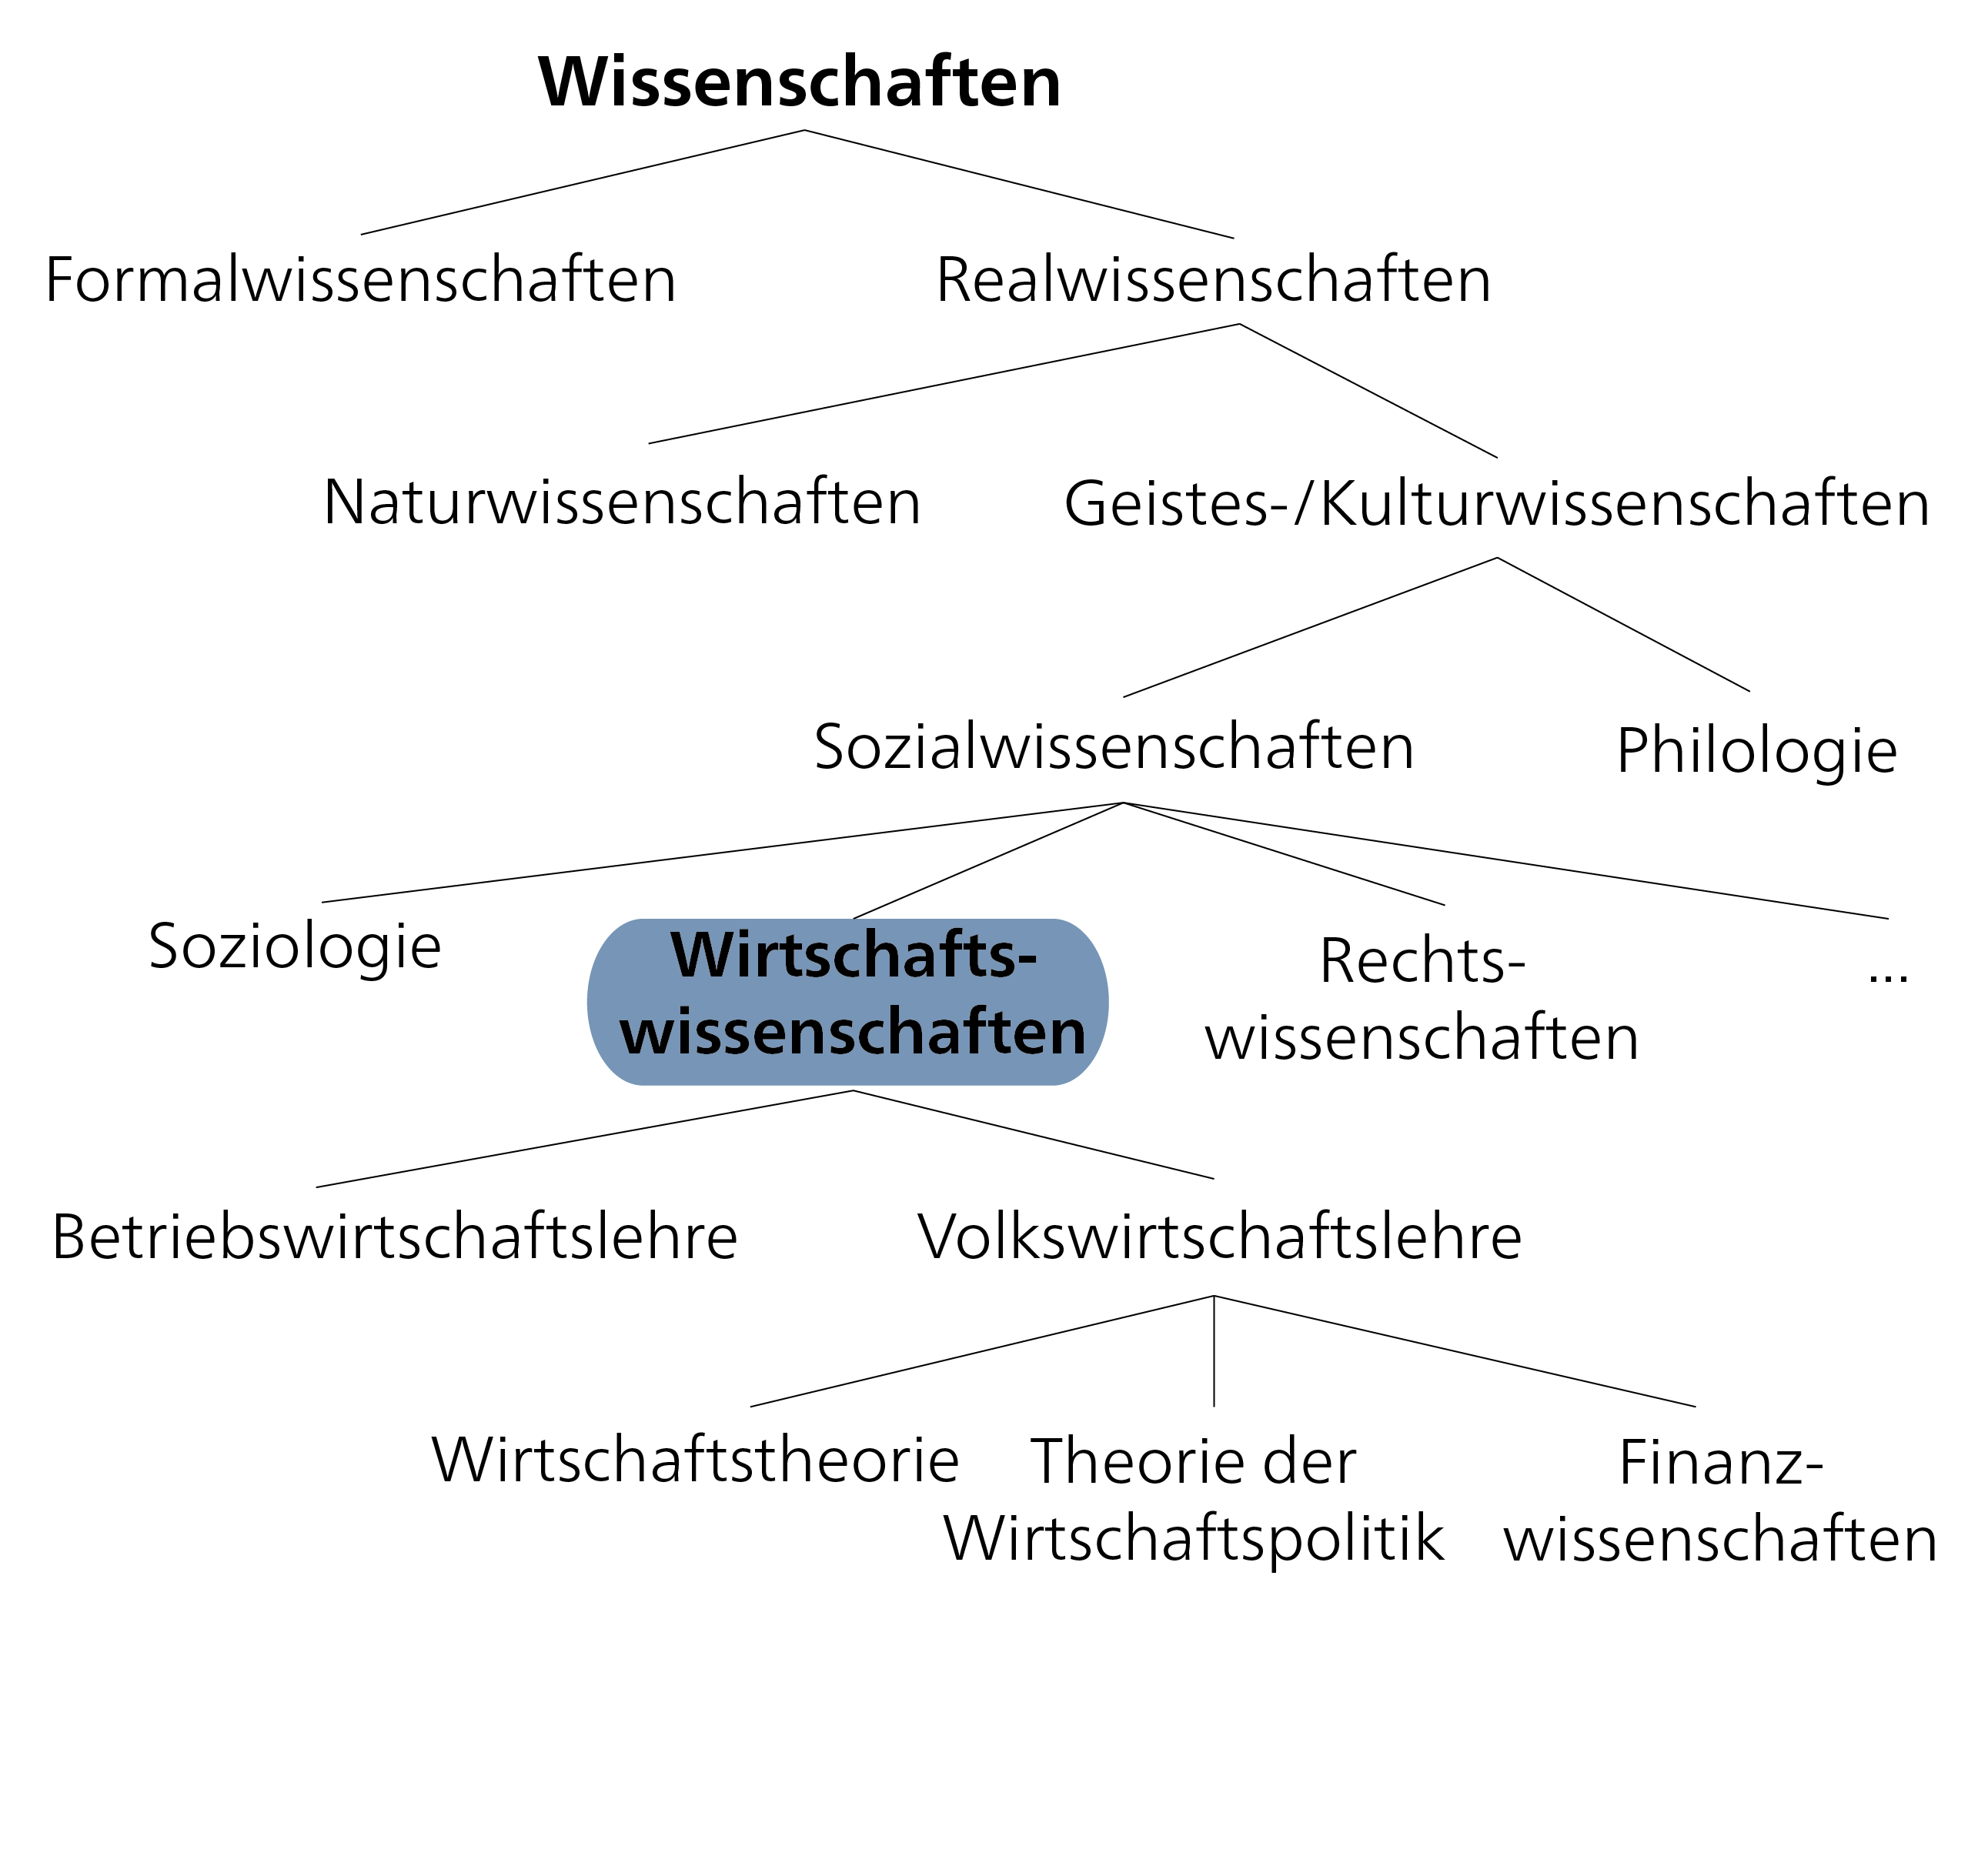
\includegraphics[keepaspectratio]{1_oekonomie-denken/images/abb1.png}}

}

\caption{Abbildung 1: Disziplinäre Verortung der
Wirtschaftswissenschaften (Engelkamp und Sell 2013, p.~3)}

\end{figure}%

\textbf{Die Betriebswirtschaftslehre} „ist die Lehre von den
wirtschaftlichen, organisatorischen, technischen sowie finanziellen
Abläufen in Unternehmen und den unterschiedlichen wirtschaftlichen
Institutionen`` (Friedli u.~a. 2019, p.~16). Darin entwickeln Forschende
eine einzelwirtschaftliche Perspektive auf den jeweiligen
Untersuchungsgegenstand.

\textbf{Die Volkswirtschaftslehre} untersucht dagegen nicht das
Geschehen innerhalb einzelner wirtschaftlicher Akteur*innen, sondern das
Zusammenspiel zwischen ihnen - also eine gesamtwirtschaftliche
Perspektive. Mit dieser Perspektive beschäftigt sich dieser Kurs.

Die Volkswirtschaftslehre lässt sich in \textbf{drei grössere
Teilbereiche} einteilen:

\textbf{Wirtschaftstheorie}: beschreibt ökonomische Theorien und deren
Implikationen. Sie unterteilt sich in die \textbf{Mikroökonomie}
(Verhalten einzelner Haushalte und Unternehmen sowie deren Abstimmung
über Märkte und Preise). Sie trifft keine Aussagen zu aggregierten
Wirtschaftszusammenhängen, sondern untersucht das Verhalten einzelner
Unternehmen und Haushalte sowie deren Abstimmungsprozess über den Markt
mithilfe von Preisanpassungen (Bontrup und Marquardt 2021, p.~1). Im
Gegensatz dazu befasst sich die \textbf{Makroökonomie} mit
gesamtwirtschaftlichen Phänomenen und Zusammenhängen von
Wirtschaftssektoren und verschiedenen Märkten. Beispielsweise werden
übergeordnete wirtschaftliche Indikatoren wie die Arbeitslosenquote oder
die Teuerung untersucht.

\textbf{Wirtschaftspolitik}: befasst sich mit staatlichen Eingriffen in
die Wirtschaft zur Steigerung der gesellschaftlichen Wohlfahrt (Bontrup
und Marquardt 2021, p.~2), etwa durch Interventionen wie Kartellverbote
oder Einführung von Mindestlöhnen.

Die \textbf{Finanzwissenschaft} untersucht die verschiedenen Komponenten
des Staatshaushalts wie Steuern oder Subventionen und deren gegenseitige
Beziehung. Dadurch werden hier implizit Fragen zur Rolle des Staates in
der Ressourcenallokation und der Einkommens- und Vermögensverteilung
untersucht.

\end{tcolorbox}

\subsection[Ökonomieverständnisse in der
Geschichte]{\texorpdfstring{Ökonomieverständnisse in der
Geschichte\footnote{Dieser kurze Überblick basiert zu Teilen auf
  (Bäuerle u.~a. 2026).}}{Ökonomieverständnisse in der Geschichte}}\label{uxf6konomieverstuxe4ndnisse-in-der-geschichte1}

Der Begriff Ökonomie taucht das erste Mal in der westlichen
Geistesgeschichte in der griechischen Antike als Lehre der
Haushaltsführung auf. Ökonomie setzt sich dabei aus zwei Begriffen
zusammen: \emph{oikos} (Haus) und \emph{nemein} (ordnen). Ökonomie
befasste sich in dem Verständnis unter anderem mit Fragen von der
Verwaltung des eigenen Besitzes, der Planung und Beurteilung
landwirtschaftlicher Tätigkeiten, der Auswahl von Sklav*innen, dem
Verhältnis von Mann und Frau. Dabei war die Ökonomie stark in Politik
und Ethik eingebettet und sollte zur Stärkung der \emph{polis}, des
Stadtstaates, beitragen. Als ultimatives Ziel stand das glückliche
Leben, \emph{eudaimonia}. Ganz im Gegensatz zur Ökonomie stand hingegen
die sogenannte Chrematistik, welche statt des glücklichen Lebens die
Geldvermehrung anstrebte und in der griechischen Antike abgelehnt wurde.

Im europäischen Mittelalter blieb das Verständnis von Ökonomie zunächst
eng mit moralischen und religiösen Vorstellungen verbunden.
Wirtschaftliches Handeln wurde nicht als eigenständiger
gesellschaftlicher Bereich verstanden, sondern war Teil einer göttlichen
und sittlichen Ordnung. Ziel wirtschaftlicher Tätigkeit war nicht die
möglichst unbegrenzte Vermehrung von Wohlstand, sondern die Sicherung
des Lebensunterhalts und das Gemeinwohl. Stark geprägt wurde dieses
Verständnis durch die Scholastik, insbesondere durch Thomas von Aquin
(c.~1225 -- 1274). Im Mittelpunkt standen Fragen nach einem gerechten
Preis (\emph{iustum pretium}), einem gerechten Lohn sowie der
moralischen Legitimität wirtschaftlicher Aktivitäten. Handel wurde
grundsätzlich akzeptiert, sofern er dem Austausch notwendiger Güter
diente. Dagegen galt die Erzielung von Gewinnen allein um ihrer selbst
willen als problematisch. Besonders kritisch wurde das Erheben von
Zinsen beurteilt, da Geld selbst als unproduktiv angesehen wurde und
nicht zur Geldvermehrung dienen sollte. Die Wirtschaft war damit stark
in ethische und gesellschaftliche Normen eingebettet.

Erst mit der Entstehung des modernen Kapitalismus, der Ausweitung des
Handels und der Industrialisierung begann sich dies zu ändern und sich
ein Verständnis von Wirtschaft als eigenständigem gesellschaftlichem
Bereich allmählich zu etablieren. Mit dem Aufstieg des
Handelskapitalismus und der Industriellen Revolution entstand im 18.
Jahrhundert die klassische politische Ökonomie. Vertreter wie Adam Smith
(1723-1790), David Ricardo (1772-1823) oder später Karl Marx (1818-1883)
interessierten sich weniger für die Verwaltung einzelner Haushalte als
für die Entstehung, Verteilung und Entwicklung des gesellschaftlichen
Reichtums ganzer Volkswirtschaften. Der Gegenstandsbereich der Ökonomie
verschob sich damit von der Haushaltsführung zur Analyse der Produktion,
Verteilung und Akkumulation von Wohlstand. Im Mittelpunkt standen Fragen
wie: Wie entsteht wirtschaftlicher Wohlstand? Wie verteilt sich das
gesellschaftliche Einkommen zwischen Arbeit, Kapital und Boden? Im
Mittelpunkt der Analysen standen gesellschaftliche Klassen -- etwa
Arbeiter*innen, Kapitalbesitzer*innen und Grundeigentümer*innen -- sowie
ihre Beziehungen zueinander. Wirtschaft wurde als gesellschaftlicher
Prozess verstanden, dessen Entwicklung durch Institutionen,
Eigentumsverhältnisse und die Verteilung des gesellschaftlichen
Überschusses geprägt wird.

Gegen Ende des 19. Jahrhunderts veränderte die sogenannte
marginalistische Revolution das Verständnis gewisser Teile der
Volkswirtschaftslehre grundlegend. Die Arbeiten von Vertretern dieser
neuen Strömung, wie bspw. William Stanley Jevons (1835-1882), Carl
Menger (1840-1921) und Léon Walras (1834-1990), bildete die Grundlage
für die Entstehung der neoklassischen Ökonomik. Im Zentrum dieser neuen
Perspektive stand nicht länger die Produktion gesellschaftlichen
Reichtums, sondern das mit Entscheidungsfähigkeit ausgestattete
Individuum. Ausgangspunkt der Analyse waren nun Haushalte und
Unternehmen, die auf Märkten unter Bedingungen knapper Ressourcen
rationale Entscheidungen treffen und ihren Nutzen beziehungsweise Gewinn
maximieren. Die Volkswirtschaft wurde als Ergebnis der Entscheidungen
vieler einzelner Wirtschaftssubjekte verstanden. Diese Veränderung
bedeutete einen grundlegenden Perspektivenwechsel. Während die
klassische politische Ökonomie die Nationalökonomie, also ganze
Volkswirtschaften ins Auge fasste und dabei gesellschaftliche Klassen,
Produktion und Verteilung in den Mittelpunkt stellte, nimmt die
Neoklassik vor allem einzelne Märkte als Bezugsrahmen und fokussierte
auf individuelle Entscheidungen und Preismechanismen. Mit den Arbeiten
von John Maynard Keynes (1883-1946) wurden Mitte des 20. Jahrhunderts
auch wieder gesamtwirtschaftliche Zusammenhänge in den Blick genommen,
nicht nur in Keynesianischen Denkschulen, sondern auch in der
Neoklassik. Aufgrund der Arbeiten von Keynes hat sich die Makroökonomie
herausgebildet.

Die Geschichte war keineswegs eine lineare Entwicklung von einem
Ökonomieverständnis zum nächsten. Oft existierten verschiedene
Verständnisse gleichzeitig, die sich gegenseitig beeinflussten,
widersprachen und sich weiterentwickelten. Die oben ausgeführten
Perspektiven sollen verdeutlichen, dass sich das Bild, was Wirtschaft
ist, mit der Zeit auch stark verändert hat und sich auch weiterhin
verändert. Zudem basieren gegenwärtige Verständnisse auf diesen
Entwicklungen, es ist also auch wichtig zu verstehen, woher gewisse
Verständnisse kommen, oder wie sie sich entwickelt haben.

\subsection{Ökonomieverständnisse der
Gegenwart}\label{uxf6konomieverstuxe4ndnisse-der-gegenwart}

Mit der Entwicklung der ökonomischen Theorien haben sich
unterschiedliche Vorstellungen davon entwickelt, was die
Volkswirtschaftslehre eigentlich untersucht. Dabei lassen sich zwei
grundsätzlich verschiedene Arten unterscheiden, wie Volkswirtschaftlehre
verstanden wird. Karl Polanyi hat diese Unterscheidung bereits 1957
gemacht (Polanyi u.~a. 1957):

\begin{itemize}
\item
  Einerseits lässt sich Ökonomie über ihren \textbf{Gegenstandsbereich
  }verstehen: Man legt fest, \emph{welchen Ausschnitt der Wirklichkeit}
  man untersucht -- unabhängig davon, mit welcher analytischen
  Perspektive. Die Medizin z. B. definiert sich über ihren
  Gegenstandsbereich: den menschlichen Körper und seine Gesundheit.
  Polanyi nennt dieses Verständnis den substantivistischen. Dieser setzt
  die Wirtschaft als empirischen Gegenstandsbereich ins Zentrum der
  Untersuchung.
\item
  Anderseits lässt sich Ökonomie über ein \textbf{spezifisches
  analytische Vorgehen} verstehen. In diesem Ansatz bildet das
  analytischen Vorgehen den Ausgangspunkt -- -- unabhängig davon,
  welchen Bereich der Wirklichkeit man damit untersucht, also unabhängig
  vom Gegenstandsbereich. Polanyi nennt dies ein formales Verständnis
  von Ökonomie. Dieses analytische Vorgehen ergibt sich einer logischen
  Herleitung aus einer empirischen Untersuchung.
\end{itemize}

Grundsätzlich definierten sich fast alle historischen Verständnisse über
die Untersuchung ihres Gegenstandsbereich. Im antiken Griechenland war
dies z. B. die Führung eines Haushalts (wie verwaltet man Land, Vorräte
und Sklaven eines Haushalts möglichst gut?). Im 17./18. Jahrhundert war
es die nationale Volkswirtschaft (wie wird ein Land als Ganzes
wohlhabend, z. B. durch Handel und Gold?). In beiden Fällen war klar
umrissen, \emph{worüber} man sprach -- ein bestimmter Ausschnitt der
Wirklichkeit.

Der gegenwärtige ökonomische Mainstream kehrt mit der marginalistischen
Revolution vermehrt von diesem Grundsatz ab und definiert sich über sein
analytisches Vorgehen und entwickelt ein formales Verständnis von
Ökonomik. Basierend auf einer Definition von Lionel Robbins aus den
1930er-Jahren wird die Ökonomik als eine Wissenschaft beschrieben, die
untersucht, wie sich Menschen unter Bedingungen von Knappheit zwischen
Alternativen entscheiden, um ihre Ziele zu erreichen. Robbins schreibt:

\begin{quote}
„Ökonomik ist die Wissenschaft, die menschliches Verhalten als Beziehung
zwischen Zielen und knappen Mitteln mit alternativen Verwendungen
untersucht`` (Robbins 1932, p.~15).
\end{quote}

Vereinfach gesagt: Ökonomik untersucht, wie Menschen mit knappen Mitteln
(Zeit, Geld, Ressourcen) möglichst gut ihre Ziele erreichen -- ganz
gleich, \emph{worum} es dabei geht, wobei es dabei fast immer um die
Maximierung des individuellen Nutzens geht. Ein einfaches Beispiel: Ein
Studierender hat am Abend nur 3 Stunden Zeit (knappe Ressource) und muss
entscheiden, ob er für die Prüfung lernt, joggen geht oder sich mit
Freunden trifft (alternative Verwendungen). Genau eine solche
Entscheidung unter Knappheit steht im Zentrum des Mainstream-Ansatzes
und bildet die analytische Ausgangslage diese Ökonomieverständnisses.
Nicht selten werden VWL-Studierende in einem Kurs in „die Grundlagen des
ökonomischen Denkens`` eingeführt. Darin geht es genau um das Einüben
dieses analytischen Vorgehens, als Grundlage der Volkswirtschaftslehre.

Aus dieser analytischen Ausgangslage wird dann das Handeln von
Akteur*innen in der Wirtschaft analysiert, wobei der Fokus stark auf
Märkten, dem Preismechanismus und nutzenoptimierenden Individuen liegt.
Märkte bilden den Rahmen in welchem Individuen versuchen durch
Entscheidungen unter Knappheit ihren Nutzen zu optimieren. Das bedeutet,
dass Fragestellung ausserhalb dieses Rahmens oft nicht Beachtung finden.
In diesem \href{https://www.youtube.com/watch?v=D-6rQmHpGfE}{Video}
spricht der Ökonom Ha-Joon Chang über das neoklassische Verständnis,
welches durch den darunterliegenden analytischen Ausgangspunkt schon
eine gewisse Ausrichtung vorgibt und gewisse Aspekte systematisch
ausblendet (siehe auch Chang und Chang 2014). Und weil dieser Ansatz
nicht an einen bestimmten Gegenstand gebunden ist, wird er in der Praxis
auch auf Themen angewendet, die man intuitiv nicht ``wirtschaftlich''
nennen würde -- etwa die Frage, warum Menschen heiraten oder Kinder
bekommen (dies wird dann als „ökonomische Entscheidung`` unter Knappheit
bspw. an Zeit, Geld und Zuneigung analysiert). 1992 bekam der Ökonom
Gary Becker für genau diese Erweiterung des Anwendungsbereichs den
Alfred-Nobel-Gedächtnispreis für Wirtschaftswissenschaften.

Viele andere Denkschulen definieren die Volkswirtschaftslehre dagegen
weiterhin über den Gegenstandsbereich: die Volkswirtschaft selbst. Sie
folgen also einem substantivistischen Verständnis. Wobei der
Gegenstandsbereich und vor allem dessen Grenzen (was gehört alles zur
Wirtschaft) unterschiedlich definiert werden können. Für Polanyi geht es
im substantivistischen Verständnis darum zu untersuchen, wie der Mensch
als Gesellschaft und in Beziehung zu seiner Umwelt die Lebensgrundlagen
bereitstellt und materiellen Wohlstand verteilt. Konkret heisst das: Es
geht um Fragen wie „Wie wird Brot produziert und verteilt?{\kern0pt}``
oder „Wer bekommt wie viel vom gesellschaftlichen Reichtum?{\kern0pt}``
-- unabhängig davon, mit welchem analytischen Vorgehen man diese Fragen
untersucht. Wie oben erwähnt gibt es aber auch unterschiedliche
Auffassungen davon, wie genau dieser Gegenstandsbereich abgegrenzt
werden soll. So betont beispielsweise die \emph{feministische Ökonomik},
dass Aktivitäten ausserhalb des Marktes, wie bspw. unbezahlte Carearbeit
ein zentraler Bereich der Ökonomie ist und unbedingt in die Analyse
einbezogen werden müssen. Die \emph{ökologische Ökonomik} betont in
ähnlicher Weise, dass die Wirtschaft in die Natur eingebettet ist, diese
die Grundlage allen wirtschaftlichen Aktivitäten bildet und so zwingend
in die ökonomische Analyse einbezogen werden muss. Entsprechend den
unterschiedlichen Verständnissen des Gegenstandsbereichs fokussieren
unterschiedliche Denkschulen auch auf unterschiedliche Aspekte, wie
bspw. auf Machtstrukturen, Institutionen oder gesamtwirtschaftliche und
gesellschaftliche Zusammenhänge und Strukturen. Im Abschnitt zur
pluralen Ökonomik (siehe 1.5) werden wir noch näher darauf eingehen, was
die neoklassische Ökonomik (Mainstream) ausmacht und einige der andern
Denkschulen näher kennenlernen.

In diesem Skript folgend wir einem substantivistischem Verständnis und
definieren Ökonomik über den Gegenstandsbereich der Ökonomie. In Kapitel
x werden wir uns dann eingehender mit diesem befassen.

\begin{tcolorbox}[enhanced jigsaw, arc=.35mm, bottomrule=.15mm, bottomtitle=1mm, breakable, colback=white, colbacktitle=quarto-callout-caution-color!10!white, colframe=quarto-callout-caution-color-frame, coltitle=black, left=2mm, leftrule=.75mm, opacityback=0, opacitybacktitle=0.6, rightrule=.15mm, title={Weiterführende Literatur}, titlerule=0mm, toprule=.15mm, toptitle=1mm]

Das Buch von Ha-Joon Chang \emph{Economics: The User's Guide} bietet
einen leichten Einstieg in Thematiken der Volkswirtschaftslehre und gibt
einen guten Überblick über die Geschichte und gegenwärtige Debatten. Je
nach Interesse können auch gut einzelne Kapitel herangezogen werden.

Chang, Ha-Joon. 2014. Economics: The User's Guide. First U.S. edition.
New York: Bloomsbury Press.

\end{tcolorbox}

\section{Geschichte des ökonomischen
Denkens}\label{geschichte-des-uxf6konomischen-denkens}

Wir haben nun kurze Einblicke in unterschiedliche Verständnisse von
Ökonomik angeschaut. In diesem Kapitel wollen wir uns noch etwas mehr
mit der Geschichte der ökonomischen Theorie auseinandersetzen und uns
fragen, wie sich die Volkswirtschaftslehre selbst entwickelt hat. Dabei
soll die Herausbildung der dominanten Denkschule, der Neoklassik, im
Vordergrund stehen.

\protect\phantomsection\label{refs}
\begin{CSLReferences}{1}{1}
\bibitem[\citeproctext]{ref-bauerleGrundfragenOkonomie2026}
Bäuerle, Lukas, Anna Katharina Keil, Rouven Reinke, und Stella Wasenitz,
Hrsg. 2026. \emph{Grundfragen Der {Ökonomie}}. 1. Auflage.
Schäffer-Poeschel Verlag.

\bibitem[\citeproctext]{ref-bontrupVolkswirtschaftslehreAusOrthodoxer2021a}
Bontrup, Heinz-J., und Ralf-M. Marquardt. 2021.
\emph{Volkswirtschaftslehre aus orthodoxer und heterodoxer Sicht}. De
Gruyter Oldenbourg.

\bibitem[\citeproctext]{ref-changLifeUniverseEverything2014}
Chang, Ha-Joon, und Ha-Joon Chang. 2014. {„Life, the Universe and
Everything. What Is Economics?``} In \emph{Economics: The User's Guide}.
Bloomsbury Press.

\bibitem[\citeproctext]{ref-engelkampEinfuehrungVolkswirtschaftslehre2013}
Engelkamp, Paul, und Friedrich L. Sell. 2013. \emph{Einführung in die
Volkswirtschaftslehre}. 6., überarbeitete und erweiterte Aufl age.
Springer Berlin Heidelberg.
\url{https://link.springer.com/10.1007/978-3-642-36522-5}.

\bibitem[\citeproctext]{ref-friedliBetriebswirtschaftslehreZusammenhangeVerstehen2019}
Friedli, Vera, Renato Müller Vasquez Callo, und Rahel Balmer-Zahnd.
2019. \emph{Betriebswirtschaftslehre: Zusammenhänge verstehen}. 4.
Auflage. Hep Verlag AG.

\bibitem[\citeproctext]{ref-polanyiEconomyInstitutedProcess1957a}
Polanyi, Karl, Karl Polanyi, Conrad M. Arensberg, und Harry W. Pearson.
1957. {„The Economy as Instituted Process``}. In \emph{Trade and Market
in the Early empires}. The Free Press \& The Falcon's Wing Press.

\bibitem[\citeproctext]{ref-robbinsEssayNatureSignificance1932}
Robbins, Lionel. 1932. \emph{An Essay on the Nature and Significance of
Economic Science}. Macmillan \& Co. Limited.

\end{CSLReferences}




\end{document}
